% vim: tw=80 cc=81 spelllang=cs spell

% XXX: Remove 'draft' in final version
% XXX: Remove 'oneside' and 'openany' for printed version
\documentclass[11pt, a4paper, oneside, openany, draft]{book}

% Input and output encoding
\usepackage[utf8]{inputenc}
\usepackage[T1]{fontenc}

% XXX: Guess what to change if you intend to write in English
\usepackage[english]{babel}

\usepackage[usenames,dvipsnames]{xcolor}
\usepackage{lmodern}
\usepackage{enumitem}
\usepackage{todonotes}
\usepackage{setspace}
\usepackage{graphicx}
\usepackage{amssymb,amsmath}
\usepackage{mathtools}
\usepackage{float}
\usepackage[pass]{geometry}
\usepackage{ifdraft}

% Theorems – add your own environments, should you need them.
\usepackage{amsthm}

% Source code listings
\usepackage[draft=false]{minted}
\usemintedstyle{friendly}
\newminted{hs}{autogobble,linenos}

% Algorithms
\usepackage[Algorithm]{algorithm}

\usepackage[ unicode=true,
             plainpages=false,
             pdfpagelabels,
             draft=false,
             hyperfootnotes=false,
             colorlinks=true,   % XXX: for PDF
             %colorlinks=false, % XXX: for print
             %hidelinks,        % XXX: for print
             linkcolor={Sepia},
             citecolor={PineGreen},
             urlcolor={MidnightBlue},
           ]{hyperref}

% XXX
\hypersetup{
    pdfauthor={Petr Kubica},
    pdftitle={...},
    pdfsubject={Master's thesis}
}

\usepackage[backend=bibtex8,
            sortlocale=en_US, % XXX
            bibencoding=UTF8
            maxnames=100
           ]{biblatex}
% XXX: Add your bibliography to bibliography.bib
\addbibresource{bibliography.bib}

\setlength{\tabcolsep}{6pt}

% Macros for linking sections suitable for use in Czech text.
% e.g., v \myref{somelabel}{sekci} → v sekci 5.2
%       v \ymref{somelabel}{kapitole} → v 5. kapitole
\newcommand{\myref}[2]{\hyperref[#2]{#1~\ref*{#2}}}
\newcommand{\ymref}[2]{\hyperref[#1]{\ref*{#1}.~#2}}

% % % % % % % % % % % % % % % % % % % % % % % % % % % % % % % % % % % % % % % %

\begin{document}
\frontmatter
% XXX: Go edit titlepage.tex
\newgeometry{margin=3cm,top=7cm}
\pagestyle{empty}

\begin{center}
    {\Large \textsc{Masaryk University}}

    {\large \textsc{Faculty of informatics}}
    \vskip4em
    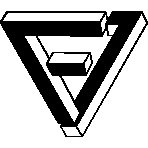
\includegraphics[width=4cm, height=4cm, draft=false] {logo_fi.pdf}
    \vskip4em
    {\begin{spacing}{1}
        \Huge \textbf{An Ahead-of-time\\Compiler for a Subset\\of TypeScript} % XXX: Title
    \end{spacing}}
    \vskip2em
    {\Large \textsc{master's thesis}} % XXX: Type
    \vskip2em
    {\LARGE \textbf{Petr Kubica}} % XXX: Author
    \vfill
    {\hfill\large Brno, 2025} % XXX: Year
\end{center}

\cleardoublepage
\restoregeometry

% XXX: Go edit frontmatter.tex
\section*{Declaration} Hereby I~declare that this paper is my original authorial work, which
I~have worked out on my own. All sources, references, and literature
used or excerpted during elaboration of this work are properly cited
and listed in complete reference to the due source.

\vspace{1cm}
\begin{flushright}
Petr Kubica
\end{flushright}

\vfill\noindent
\textbf{Advisor:} RNDr. Petr Ročkai, Ph.D.   % XXX
% \\\textbf{Konzultant:} nope % XXX
\cleardoublepage

\section*{Acknowledgements} % XXX
I would like to thank everyone who has helped me make this thesis possible, especially my advisor Petr Ročkai for his guidance and advice. I would also like to thank my friends and colleagues, particularly from the ParaDiSe laboratory, for their support. To anyone negatively affected by my lack of time for other work and activities, I apologize and thank you for your understanding. Finally, I would like to thank my family for their support.
\cleardoublepage

\section*{Abstract} % XXX
This thesis describes the design and implementation of an ahead-of-time compiler for a subset of TypeScript. The compiler is implemented as an extension of Jaculus-machine -- a small, embeddable JavaScript runtime environment. The compiler makes use of TypeScript's type annotations to generate more monomorphic code than what is possible by using JavaScript. It can compile parts of an input program to machine code, which can be used to improve its performance. The compiler is then evaluated on several benchmarks and compared to only using an interpreter.

\subsection*{Keywords} % XXX
JavaScript, TypeScript, compiler, ahead-of-time compilation, embedded systems
\cleardoublepage


\setcounter{tocdepth}{2}
\tableofcontents
\pagestyle{plain}

\mainmatter

\chapter{Motivation}

Traditionally, microcontrollers are programmed in compiled languages such as C or C++. These languages offer high performance and low-level access to hardware, which is important in many embedded applications. However, they can be also difficult to learn and use, especially for beginners.

At Robotárna, a branch of Leisure Center Helceletka in Brno, we teach programming of microcontrollers to teenagers. To make the learning process easier, we have decided to use a high-level interpreted language -- JavaScript -- instead. While this approach is unconventional, it has a strong advantage of a very fast code-build-test cycle. The speed of this cycle makes it easier for students to maintain their focus and allows them to experiment more with their code.

So far, we have observed success with this approach. We see students being able to learn the basics faster and start working on more interesting projects sooner. However, with students creating more complex projects, we have also reached a point where we need to consider performance JavaScript programs.

JavaScript, as an interpreted language, suffers from the inherent flaw of slow execution speed. It comes as a cost for the ease of use of JavaScript and, in a large part, stems from its dynamic nature and the difficulty to implement optimizations. Occasionally, more capable students encounter the lower performance of JavaScript as a limitation and have difficulties to implement their ideas.

Because programming in JavaScript as a dynamically typed language can sometimes lead to errors that are difficult to debug, we usually do not write JavaScript directly. Instead, TypeScript is used and compiled to JavaScript only before execution.

What is of particular interest, is the fact, that at the time of compilation to JavaScript, type annotations are removed from the input program, and some information about the input program is lost. This fact is unfortunate, because the type information could be used by the runtime environment to perform simple optimizations when loading the program.

In this thesis, we will explore the possibility of using a slightly modified subset of TypeScript as the input of our runtime. We will use the type information to identify segments of code that can be easily compiled to machine code and replace them with their machine code equivalent.

We believe, this will lead to a significant improvement in performance of some parts of such input programs that are written specifically, so they can benefit from this optimization.

\chapter{Overview}

The goal of this thesis is to implement a simple compiler for a subset of TypeScript. This chapter describes, high-level architecture of the compiler, and related technologies used or considered for its implementation.

\section{Requirements}

The proposed compiler will be primarily used in restricted environments, such as microcontrollers. For this reason, the compiler must be small and resource efficient. The compiler will be used as a part of the JavaScript runtime Jaculus (described in Section \ref{jaculus}).

Because the compiler should be simple, it will only perform static analysis and compilation of selected parts of the input program. After the compilation is completed, the compiler will not perform any further work during the execution of the program. The compilation will be performed at the level of functions. If more suitable functions are found in a single file, they will be compiled together and statically linked together.

The compiler must be able to compile such subset of TypeScript, which will make it possible to write useful subroutines that can make use of the increased performance of compiled code. Initially, the compiler will support only a small part of the language, but it should be possible to extend the compiler in the future.

Examples of programs that should be able to take advantage of the compiler are:
\begin{itemize}
    \item mathematical functions,
    \item functions for graphical rendering.
\end{itemize}

\section{Architecture}

The compiler is separated into multiple parts. Each part is responsible for a single step of the compilation process. The compiler is designed to depend on external libraries as weakly as possible. This means that it is possible to replace these libraries with other implementations without an extensive rewrite of the compiler (particularly the compiler backend MIR, and JavaScript engine QuickJS).

\todo{add a diagram of the architecture}


\section{Related technologies}

Several other projects were used for the implementation of the proposed compiler. These projects are described in this section. This section also describes multiple small compiler backends which were considered as candidate options.

\subsection{Jaculus}\label{jaculus}

Jaculus was originally created as a part of the author's bachelor's thesis\cite{jaculusthesis}. This work is a continuation of the project.

Jaculus is a platform for programming microcontrollers using JavaScript. At core, Jaculus uses the QuickJS JavaScript engine. Jaculus' core library, Jaculus-machine, is of particular interest for this work, as the proposed compiler is implemented as an extension of this library. Jaculus-machine implements high-level C++ abstractions around QuickJS and implements some core features for the runtime (e.g., an event loop).

\subsection{QuickJS}

QuickJS is an embeddable JavaScript engine. The version used in the current version of Jaculus-machine implements the ECMAScript 2020 Language Specification\cite{ecma262}.

QuickJS is designed to have a small code and memory footprint, and to be easily embeddable in larger programs. An important target of QuickJS is to have a very short startup time.

QuickJS uses a stack-based bytecode machine. To speed up the startup time, QuickJS generates bytecode while parsing the source code without the use of an intermediate representation or AST. Some simple optimizations are then performed on the generated bytecode.

Values in JavaScript have a dynamic type, which may fall in several categories. In QuickJS, values are represented using a tagged union -- a structure with two 64-bit values representing the tag and a corresponding value.

Some primitive values are placed directly into this structure while others are allocated on the heap and the structure only contains a pointer to the value. Values which require memory allocation use reference counting with cycle detection for memory management.

\todo{expand}


\subsection{Compiler backends}

\todo{write}

\subsubsection{MIR}

MIR is a small compiler backend designed for usage in JIT scenarios.

\chapter{Language description}\label{language}

The language implemented by the compiler is, at core, a subset of JavaScript with added type annotations and slightly modified semantics of arithmetic operations. This, in a way, makes it a subset of a modified TypeScript.

The used version of JavaScript is standardized in the ECMAScript 2020 Language Specification\cite{ecma262}. This document serves as the primary reference for the language implemented by the compiler.

TypeScript, on the other hand, does currently not have a formal standard and relies on an official implementation which serves as a reference. The last version which had a formal specification was version 1.8\cite{typescript18}. This version serves as a reference for the extended grammar and semantics of our language.

While this chapter describes the full language we would like to implement, only a part of this language is currently supported by the compiler. The language features that are supported by the compiler are described in a later chapter.\todo{link}

\section{Grammar}

The language grammar extends the grammar defined in the ECMAScript 2020 Language Specification\cite{ecma262} by allowing the writing of type annotations in function signatures and declarations of variables. A type annotation is defined by the following production:

\begin{minted}{text}
    TypeAnnotation -> : Identifier
\end{minted}

\todo{add productions, fix grammar form, template parameters}

The declarations of variables and type annotations then follow the following modified productions:
\begin{minted}{text}
    VariableDeclaration -> BindingIdentifier TypeAnnotation[opt] Initializer[opt]
    VariableDeclaration -> BindingPattern Initializer[opt]

    LexicalBinding -> BindingIdentifier TypeAnnotation[opt] Initializer[opt]
    LexicalBinding -> BindingPattern Initializer[opt]

    SingleNameBinding -> BindingIdentifier TypeAnnotation[opt] Initializer[opt]
\end{minted}
\todo{false}

\section{Language semantics}

The semantics of the implemented language are the same as described in the ECMAScript 2020 Language Specification\cite{ecma262} except for the cases described below\todo{TypeScript}.

Because the values in JavaScript are untyped, many operations on them start with a type check and the selection of correct behavior of the operation. With statically typed variables, however, we can perform this selection at compile time and speed up the program execution. It is therefore advantageous to define these operations in such a way that the result type is always the same independently on the input values. We can also often replace the typical type union, which used to represent a JavaScript value, with the value itself.

Because many microcontrollers do not have a 64-bit FPU\footnote{FPU: floating-point unit}, it is also desirable to avoid floating point operations. Unfortunately, in JavaScript, the number type is said to be an IEEE 754-2019 double precision float\cite{ieee754}. Many interpreters, including QuickJS, use an integer type (typically a 32-bit int) to represent some values of the \texttt{number} type as an optimization, however, when the result of an operation does not fit in this type, the operands have to be promoted to a floating point number and the operation is performed in the floating point domain. Even if a program is written so that no floating point operations are performed, this approach still has two downsides:
\begin{itemize}
    \item every arithmetic operation contains an overflow check, and
    \item the \texttt{number} type has to be a type union.
\end{itemize}

It is therefore a good idea to define a new primitive type \texttt{Int32} which guarantees that all arithmetic operations with two \texttt{Int32} operands will result in a new value of the same type. The \texttt{Int32} type can be used in any other context where the specification\todo{how to abbrev?} expects a value of the type \texttt{number}. In such cases, the value will behave the same as an equivalent value of the type \texttt{number}.

\todo{implicit conversions on assignment}

\todo{explicit conversions (not implemented yet)}

\todo{linkage}


\todo{TypeScript -- types are not nullable}

\section{Supported features}



% As we want to implement an ahead-of-time compiler for Jaculus, there are only two obvious language options to choose from -- JavaScript and TypeScript. JavaScript is the native language used by the internal JavaScript interpreter while TypeScript support is provided by tools on the programmer's device.

% The ahead-of-time compiler should be able to perform simple static analysis of the input program, select parts that can be easily compiled into machine code, and replace these parts with its machine code equivalent. This whole process should preferably happen as fast as possible as the compiler will be running in an environment with limited computational resources. The machine code should also be reasonably well performant, given the constrained environment.

% The main feature that sets the available languages apart is their typing system. While JavaScript is dynamically typed, TypeScript uses gradual typing. In a gradual typing system, some variables have a static type known at compile time, while other variables may have an unknown, dynamic type (in TypeScript called \texttt{any}).

% Static types are an advantageous feature when writing a compiler, as they can help the compiler generate faster code without requiring complex heuristics. For this reason, we have elected to use a subset of TypeScript as the language supported by our compiler. A specification of supported language features is described later in Section ?\todo{add link}.

% Because TypeScript is a strict superset of JavaScript, most of its semantics comes from JavaScript, or more formally ECMAScipt, as specified in the ECMAScipt Language Specification\cite{ecma262}. This thesis will therefore often refer to the JavaScript specification for the semantics of operations. TypeScript, unfortunately, has no formal specification since version 1.8. Since then, it relies on the official implementation which serves as a reference.

\chapter{Intermediate Representation}

The proposed compiler works in multiple stages and uses different representations for the products generated by each stage. This chapter describes the first intermediate representation which is generated from an AST.

In the intermediate representation, the input program is split into individual functions. The intermediate representation represents a function in the form of a control-flow graph (CFG). A CFG typically consists of basic blocks which form small chunks of linear code. Each basic block ends with a terminator instruction which can either perform a (conditional) jump to a different basic block, or terminate the whole function. Together, basic blocks (nodes) with jump instructions (edges) form a directed graph which represents all possible paths through the program.

The semantics of the program described using the intermediate representation is defined in the form of an abstract virtual machine which can execute this code.

\section{Virtual machine semantics}

The virtual machine consists of:
\begin{itemize}
    \item program code,
    \item an instruction pointer,
    \item an unlimited number of virtual registers,
    \item a cleanup stack, and
    \item a reference to a JavaScript virtual machine instance.
\end{itemize}

The virtual machine can execute a single function with the given call arguments. Each step of the execution performs a single instruction at the position of the instruction pointer and updates the instruction pointer accordingly. A \texttt{Call} instruction is not processed by the same machine. Instead, the virtual machine is paused until the call is finished by the correct means (e.g., as a native call, in a new virtual machine).

To simplify the process of generating the IR, the virtual machine uses an unlimited number of virtual registers. These will be referred to as \textit{IR registers}. IR registers should not be confused with machine registers, as they can hold different, in some cases complex, value types, which are only later mapped into the physical memory or registers. IR registers are statically typed and can take on the types described in Section \ref{ir:types}. Each register has a unique identifier represented by a numeric value.

A cleanup stack is a piece of memory which allows the program to simplify the management of value ownership. When the reference count of a value should be reduced, it is not done directly because more complex analysis of the usage of the value would be necessary. Instead, the value is placed onto the cleanup stack and its reference count is reduced at the exit of the function.

Some instructions need to interact with the underlying JavaScript virtual machine to perform the operation which they represent. A reference to the JavaScript virtual machine must be therefore accessible. The model does not specify how the JS VM will be available, but two possible approaches would be:
\begin{itemize}
    \item a constant in static memory - a function is bound to a JS VM at compile time, or
    \item through a function parameter - a function may be shared with multiple JS VMs.
\end{itemize}


\section{IR Types}\label{ir:types}

The types used by the IR are chosen as a middle point between standard JavaScript types and typical native types. This allows some primitive types to be represented without the need of a "tag" to distinguish between different types available in JavaScript which can lead to a faster runtime performance and smaller memory usage. Some newly introduced primitive types can also provide faster implementation of, for example, arithmetic operations at the cost of not conforming with the ECMAScript specification. The list of available types can be seen in Table \ref{tab:types}.
\todo{move part to language specification}

\begin{table}[H]
    \centering
    \begin{tabular}{l | l}
        Type name   & Possible values                                                \\\hline
        \texttt{Void}        & the JavaScript value \texttt{undefined}                        \\
        \texttt{Int32}       & Signed 32-bit integer number                                   \\
        \texttt{Float}       & IEEE 754-2019 double-precision floating point number          \\
        \texttt{Bool}        & true/false                                                     \\
        \texttt{Object}      & Reference to a JavaScript Object (primitive type not \\
                             & allowed)  \\
        \texttt{StringConst} & Reference to a static string value                             \\
        \texttt{String}      & Reference to a reference-counted string value                  \\
        \texttt{Any}         & Value of JavaScript's dynamic type (type union)
    \end{tabular}
    \caption{Possible types of intermediate registers}
    \label{tab:types}
\end{table}


\section{IR Instructions}

IR instructions represent simple operations and may have different variants based on types of their operands. These operations correspond to different operations from the modified JavaScript as described in a later section\todo{link our js specification}. There are four kinds of instructions:


\texttt{Operation} represents a simple instruction with up to three operands (typically 2 inputs and 1 output) and may perform different operations depending on their argument types. All operands must be IR registers, or must be ignored by a given instruction.

\texttt{ConstInit} performs a constant initialization of an IR register. They only have two operands - an IR register, and an immediate value. The types of these values correspond to primitive value literals - i.e., Bool, Int32, Float, StringConst.

\texttt{Call} represents a function call. These can have a variable number of parameters and can describe a native function call or JavaScript function call. All operands representing arguments and return target must be IR registers. The call target may either be a string identifier of a native function, or an IR register containing a function object\todo{not implemented}. The types of IR registers representing arguments and return value must correspond to the respective types defined in the signature of the called function.

\texttt{Terminator} terminates a basic block. They can be used to describe control flow.


\begin{table}
    \centering
    \begin{tabular}{l | l | l}
        \texttt{Opcode}      & Signature \texttt{(a b -> res)}    &  Meaning                    \\\hline
        \texttt{Add}         & \texttt{a      a     -> a        } &  Addition                   \\
        \texttt{Sub}         & \texttt{a      a     -> a        } &  Subtraction                \\
        \texttt{Mul}         & \texttt{a      a     -> a        } &  Multiplication             \\
        \texttt{Div}         & \texttt{a      a     -> a        } &  Division                   \\
        \texttt{Rem}         & \texttt{a      a     -> a        } &  Remainder                  \\
        \texttt{Pow}         & \texttt{a      a     -> a        } &  Exponentiation             \\
        \texttt{LShift}      & \texttt{Int32  Int32 -> Int32    } &  Left shift                 \\
        \texttt{RShift}      & \texttt{Int32  Int32 -> Int32    } &  Right shift                \\
        \texttt{URShift}     & \texttt{Int32  Int32 -> Int32    } &  Unsigned right shift       \\
        \texttt{BitAnd}      & \texttt{Int32  Int32 -> Int32    } &  Bitwise AND                \\
        \texttt{BitOr}       & \texttt{Int32  Int32 -> Int32    } &  Bitwise OR                 \\
        \texttt{BitXor}      & \texttt{Int32  Int32 -> Int32    } &  Bitwise XOR                \\
        \texttt{Eq}          & \texttt{a      a     -> Bool     } &  Equality                   \\
        \texttt{Neq}         & \texttt{a      a     -> Bool     } &  Non-equality               \\
        \texttt{Gt}          & \texttt{a      a     -> Bool     } &  Greater than               \\
        \texttt{Gte}         & \texttt{a      a     -> Bool     } &  Greater-or-equal           \\
        \texttt{Lt}          & \texttt{a      a     -> Bool     } &  Less than                  \\
        \texttt{Lte}         & \texttt{a      a     -> Bool     } &  Less-or-equal              \\
        \texttt{GetMember}   & \texttt{parent id    -> Any      } &  Get member                 \\
        \texttt{SetMember}   & \texttt{id     a     -> parent   } &  Set member                 \\
                             & \texttt{id = StringConst | Int32 } &                             \\
                             & \texttt{parent = Object | Any    } &                             \\
        \texttt{Set}         & \texttt{a      \_    -> b        } &  Set IR register, convert   \\
        \texttt{BoolNot}     & \texttt{a      \_    -> Bool     } &  Logical negation           \\
        \texttt{BitNot}      & \texttt{Int32  \_    -> Int32    } &  Bitwise negation           \\
        \texttt{UnPlus}      & \texttt{a      \_    -> Number   } &  Unary plus                 \\
        \texttt{UnMinus}     & \texttt{a      \_    -> a        } &  Unary minus                \\
        \texttt{Dup}         & \texttt{a      \_    -> \_       } &  Increment reference count  \\
        \texttt{PushFree}    & \texttt{a      \_    -> \_       } &  Push to the cleanup stack  \\
    \end{tabular}
    \caption{Table: List of Operations. The column signature shows the possible types of IR registers used as operands. Most Operations have three operands - two inputs and one output. Therefore, the three operands are denoted as \texttt{a b -> res}. Type placeholders are used to show all possible overloaded variants of a given Operation. The placeholder \texttt{\_} describes an unused operand. The syntax \texttt{id = StringConst | Int32} describes a type alias \texttt{id} which can take on the listed types (\texttt{StringConst} or \texttt{Int32}). }
    \label{tab:opcodes}
\end{table}

The arithmetic Operations implement the operations as described in Chapter \ref{language}.

The Operations \texttt{Dup} and \texttt{PushFree}\footnotemark[1] are used for updating the reference counts\footnotemark[2] of JavaScript values. To simplify the process of decreasing the reference counts, a cleanup stack is used at runtime. The \texttt{Dup} instruction immediately increments the reference count of a value, whereas the \texttt{PushFree} instruction only pushes the value to the "cleanup" stack, which is used in function's epilogue to decrease the reference counts of all values used during it runtime. To create an equivalent machine code, numeric values should be represented as \texttt{Float}, or \texttt{Any}\todo{not implemented}\footnotemark[3].

\footnotetext[1]{The names \texttt{Dup} and \texttt{Free} are not entirely descriptive of the operation which they perform, however, an equivalent operation in QuickJS is performed by a pair of functions \texttt{JS\_DupValue} and \texttt{JS\_FreeValue}, from the names are adapted.}

\footnotetext[2]{While we talk about reference counts of values, the interface is not limited to this memory management approach. In practice, the underlying JavaScript interpreter may use a different algorithm (such as mark-and-sweep). In essence \texttt{Dup} and \texttt{PushFree} instructions only describe the action of taking and releasing the ownership of a value.}

\footnotetext[3]{The performance of arithmetic operations on different types may vary depending on the target CPU - for example, on a 32-bit CPU without 64-bit float acceleration, work with small integer values will be significantly faster when the \texttt{Any} type is used instead of \texttt{Float}.}


\section{IR interpreter}

An interpreter for the intermediate representation is available as a part of the test suite to allow for testing of the generated IR without compiling it to the native code. It allows for catching IR generation errors early and for avoiding the debugging of the final machine code. The interpreter works directly with the immediate variables and keeps track of their types and reference counts\todo{extend for primitives} during the runtime.

\chapter{Implementation}

The compilation pipeline consists of multiple phases. The input is the content of a single TypeScript file, and the output is runnable JavaScript code with stubs referring to generated native functions.


\section{Parser}

\todo{tokenization}
The first phase of the compilation pipeline involves parsing the input source code. The TypeScript code is converted to an abstract syntax tree (AST) using a recursive descent parser. The design of the parser is inspired by the parser described in the book \textit{Crafting Interpreters}\cite{craftinginterpreters}.

Recursive descent parser is a top-down parser from the family of LL parsers. It is usually implemented by transforming each grammar rule into a function. When a function for a rule is called, it tries to match the input against the rule by recursively calling the functions for its sub-rules.

While recursive parsers are easy to implement and understand, they are not able to parse all grammars. In particular, they cannot parse grammars with left recursion. Because the language grammar, as described in Section \ref{lang:grammar}, is left recursive slight modifications to the grammar and the algorithm are needed.

Infix binary expressions are a case of left recursion in the grammar. They are instead parsed using a cover grammar which is later refined into the correct expression tree. In general, a cover grammar is a more general grammar which is easier to parse but may not produce an equivalent parse tree. The cover grammar is then refined into the correct parse tree using a separate algorithm. The cover grammar used for parsing infix binary expressions is defined as follows:

\todo{fix typesetting iteration}
\GrammarRule[BinaryExpression]{}{
    \nonterminal[UnaryExpression]{}{} \gramiter{\nonterminal[InfixBinaryOperator]{}{} \nonterminal[UnaryExpression]{}{}}
}

The result is a flat representation of the expression without regard to the operator precedence and associativity. It is then refined to the correct expression tree using Shunting Yard algorithm\cite{algol60}.

Another case of left recursion in the grammar are the non-terminals \nonterminal[MemberExpression]{}{} and \nonterminal[CallExpression]{}{}. In both cases, there are multiple productions with left recursion. Fortunately, all of these productions represent a repeated application of a rule. Therefore, they can be parsed iteratively and then transformed into a correct AST. The non-left recursive productions are always applied first, and the left recursive productions are applied in a loop until no more productions can be applied. The grammar for these two non-terminals is defined as follows:

\GrammarRule[MemberExpression]{Yield, Await}{
    \nonterminal[SuperProperty]{?Yield, ?Await}{} \\
    \nonterminal[MetaProperty]{}{} \\
    \nonterminal[PrimaryExpression]{?Yield, ?Await}{} \\
    \terminal{new} \nonterminal[MemberExpression]{?Yield, ?Await}{} \nonterminal[Arguments]{}{} \\
    \nonterminal[MemberExpression]{?Yield, ?Await}{} \terminal{[} \nonterminal[Expression]{?Yield, ?Await}{} \terminal{]} \\
    \nonterminal[MemberExpression]{?Yield, ?Await}{} \terminal{.} \nonterminal[IdentifierName]{}{} \\
    \nonterminal[MemberExpression]{?Yield, ?Await}{} \terminal{.} \nonterminal[PrivateIdentifier]{}{} \\
    \nonterminal[MemberExpression]{?Yield, ?Await}{} \nonterminal[TemplateLiteral]{}{}
}

\GrammarRule[CallExpression]{Yield, Await}{
    \nonterminal[CoverCallExpressionAndAsyncArrowHead]{?Yield, ?Await}{} \\
    \nonterminal[SuperCall]{?Yield, ?Await}{} \\
    \nonterminal[ImportCall]{?Yield, ?Await}{} \\
    \nonterminal[CallExpression]{}{} \nonterminal[Arguments]{}{} \\
    \nonterminal[CallExpression]{}{} \terminal{[} \nonterminal[Expression]{?Yield, ?Await}{} \terminal{]} \\
    \nonterminal[CallExpression]{}{} \terminal{.} \nonterminal[IdentifierName]{}{} \\
    \nonterminal[CallExpression]{}{} \terminal{.} \nonterminal[PrivateIdentifier]{}{} \\
    \nonterminal[CallExpression]{}{} \nonterminal[TemplateLiteral]{}{}
}

The remaining left recursive productions represent simple lists of items and can be, again, parsed iteratively. These non-terminal are: \nonterminal[FormalParameters]{}{}, \nonterminal[Expression]{}{} (comma operator), \nonterminal[LexicalDeclaration]{}{}, \nonterminal[VariableDeclaration]{}{}, \nonterminal[Arguments]{}{}, and \nonterminal[StatementList]{}{}.


\section{Generating the intermediate representation}

After parsing the input source code, the compiler generates an intermediate representation (IR) of the program. The IR is described in detail in Chapter \ref{ir}.

The IR generator traverses the AST and collects all top-level function declarations. From these functions, those suitable for compilation are selected for further processing. The selected functions are then compiled to the IR.

Every function in the AST consists of two parts: a signature and a body. First, the IR generator iterates over all function declarations and creates a list of all possibly compilable functions. In this step, a function is considered compilable if the function signature contains type annotations for all parameters and the return type. The list allows the generator to determine which functions are to be compiled and to insert native calls in relevant places. Then, the function bodies are processed independently on a per-function basis. If compilation of one of these functions fails, the entire compilation process fails with a \texttt{SyntaxError} exception and the input program cannot be executed.

The statements in the function body are recursively traversed by the compiler and the AST is transformed into the intermediate representation described in Chapter \ref{ir}.

The IR generator is implemented as a number of functions which describe the generation process for different AST nodes. These functions keep track of the context of IR generation, in particular, lexical and variable declarations and their scopes, the active basic block, break and continue targets, and the rest of the CFG that is being created.\todo{?}

There are two kinds of AST nodes that generate a part of the IR code -- statements and expressions. When an AST node is being processed, all of its children get processed recursively. In the case of expressions, the sub-nodes have a value result, which may be used by the parent node in some way. The results can have different value types and can be used in different ways. Some may be used as assignment targets (\textit{l-values}) and some may be only used as value operands in another expression (\textit{r-values}). When l-values are to be used as value operands in another expression, they first have to be evaluated (their value is acquired).

The resulting value type of some AST node can not be determined by the node type alone, and depends on the subtree of the node. For example, a \nonterminal[PrimaryExpression]{}{} node may represent a variable (an l-value) or a literal (an r-value). The IR generator therefore first generates the IR code for the sub-nodes and only then determines the value type of the node.

Sometimes, the final value type of evaluated sub-node may be incompatible with what the parent node expects. In these cases, the input code contains syntax error, because static semantics of the language are violated. The IR generator will then throw a \texttt{SyntaxError} exception and abort the compilation process.

When a value is saved into an IR register, its reference count needs to be updated. This operation is implemented by a \texttt{Dup} instruction which is emitted. The reference count needs to be decreased after the value is no longer needed. To avoid analyzing the code and finding the correct places to perform this task, the value is saved using the \texttt{PushFree} instruction and the reference count is decreased before returning from the function.

The process of generating the IR code itself can be viewed as two simple cases -- linear code, and branching code. Generating linear code is trivial, as the respective AST nodes are simply replaced by their counterparts consisting of IR instructions. These can be directly emitted to the currently active basic block.

When generating branching code, the active basic block has to be split into two parts -- entry, and exit. The entry block contains the original code without a terminator instruction while the exit block retains only the terminator instruction. The branching code is then simply emitted into the entry block and a number of newly created blocks for all new paths. Paths that do not terminate, or contain non-linear\todo{check} control flow (i.e., \texttt{break} or \texttt{continue} statements) must all converge to the exit block.

\subsection{Examples of IR generation}

\todo{show the IR-gen of some significant AST nodes -- linear expression, if, for, short-circuit expression, terminating statement}

\subsection{Runtime requirements of IR function}\todo{find a better title}\label{subsec:irruntime}

There are very few requirements on how a function represented by the intermediate representation should behave. The values in IR registers can be stored in any way, be it in CPU registers, in stack memory, or in a different way. There is also no standardized calling convention. The execution environment must only arrange for the function arguments to be passed to the correct IR registers, and the return value to be passed back to the caller.\todo{move to IR chapter?}

A function in the IR requires access to the instance of the JavaScript interpreter it runs under. To implement the \texttt{PushFree} instruction, it also needs a secondary stack (or another container) for storing all values that need to be freed at exit.


\section{Compiler backend}

The compiler relies on the MIR compiler backend to perform register allocation, code generation, and optimization of the machine code. MIR generates functions with a standard calling convention for target platform.

The signature of generated functions is not compatible with the signature of functions callable from QuickJS. Therefore, for every compiled function, a companion function with a compatible signature is generated.

The MIR code is generated by simply replacing parts of the IR with the respective MIR representation. Some simple instructions can be replaced by a single MIR instruction, some more complex are replaced by multiple MIR instructions or a function call.

The final, native, functions require a runtime context, as described in Section \ref{subsec:irruntime}. The context primarily contains a pointer to an instance of the JavaScript interpreter. It also contains a secondary stack used by the \texttt{PushFree} instruction. Lastly, it stores an information about whether an exception has occurred in the function.

Some instructions and function calls may result in a JavaScript exception. For these, additional checks are inserted into the MIR code. These checks use the exception flag in the runtime context to determine whether an exception has occurred. If an exception occurs, the function returns a default value and the exception flag is set. The caller of the function then checks the exception flag and propagates the exception further up the call stack.

These functions are statically bound to a single JavaScript runtime and can not be shared between multiple runtime instances. This allows the functions to use the same runtime context through a constant pointer that is linked to them at compilation.


\section{Stubs}\label{impl:stubs}

After compiling the functions to native code, they need to be made accessible to the interpreter. The compiled functions are therefore wrapped in JavaScript function objects (stubs) which, when called from JavaScript, perform a native call to the compiled function. They are then defined as properties of JavaScript's global object\footnotemark[1] with unique identifiers.

\footnotetext[1]{In JavaScript, a global object is a special object \texttt{globalThis} which is globally accessible from an execution context (i.e., including different modules). Properties of the global object are a part of the lexical scope, and one of its functions is to provide intrinsic objects and values to the execution environment.}

New JavaScript source code is also generated. In this source code, the original declarations of compiled functions are replaced by references to the stubs, and by comments with the original function's source code.

JavaScript applies declaration and value hoisting on function declarations. This means that in a standard JavaScript program, it is possible to reference and use a function before it is declared. In the newly generated code, we can only replicate this behavior by declaring a new function which would call the stub function. Declaring a new function would result in another level of indirection in every call of this function and induce unnecessary overhead.

As maintaining JavaScript's behavior is, in this case, not feasible without modifying the underlying interpreter, we have elected to change the behavior instead. For declaring the aliases for the stub functions, we use a constant lexical declaration (i.e., \texttt{const}). While the runtime semantics is slightly different, its also disallows users from rebinding the same name to a different function (or value). Such behavior would be potentially dangerous, because at compile time functions are statically linked to each other. If the user rebound a function name which was referenced from a different compiled function, they might expect a change in behavior of the compiled function which would, however, not happen. By declaring the function reference as \texttt{const}, such code would result in a syntax error instead.


\section{Interpreter}

The newly generated JavaScript code is then executed by the QuickJS interpreter. The interpreter is not modified and is used through the Jaculus-machine abstraction layer. After preprocessing the source code, as described in Section \ref{impl:stubs}, and defining new properties of the JavaScript's global object, the new JavaScript code is executed as normal.

\section{Integration with Jaculus-machine}

Jaculus-machine uses a modular approach which allows the programmer to select which modules should be a part of a JavaScript runtime (called \textit{Machine}). Jaculus-machine calls these modules \textit{MFeatures}. The configuration of a selected set of MFeatures is performed at compile time which allows the individual MFeatures to interact with one another without significant overhead caused by dynamic bindings.

The compiler implementation is provided as a single MFeature, which provides a method \texttt{eval} for executing input source code. The source code is always processed by the compiler and the generated code is executed.

\chapter{Evaluation}

\section{Comparison with interpreted code}

The main reason for adding a compiler into a JavaScript runtime is a potential increase in execution speed. This section evaluates the performance difference between using Jaculus-machine with, and without the newly added compiler.

To measure the performance difference, we choose several benchmarks which aim to test various language constructs.

\section{Methodology}

Because Jaculus primarily targets resource-limited environments, the benchmarks were executed on a Raspberry Pi 3 Model B\cite{rpi3b_product} single board computer (SBC). The SBC is equipped with a 64-bit quad-core ARM Cortex-A53 CPU running at 1.2 GHz and 1 GB of RAM. The CPU is based on the ARMv8-A architecture and uses the AArch64 instruction set which is supported by the MIR backend used in the compiler.

The CPU has a 64-bit floating-point unit (FPU) and will probably not take the full advantage of our extension of JavaScript which allows programs to use integer operations instead of IEEE 754 floating-point operations.

A benchmarking executable was added to Jaculus-machine which allows the user to execute a JavaScript file in an interpreter or a compiler mode. The executable can specify the number of iterations to run, and can define global constants available from the interpreter to parameterize the benchmark. In each iteration, a new instance of the Jaculus-machine is created, and the benchmark is executed. The time taken to execute the benchmark is measured using the \texttt{time} command in a Linux shell.

The code being run in the interpreter and compiler modes is not identical because the interpreter does not support the added type annotations. The compiler, however, requires them to be present in the code. The code for both benchmarks therefore contains small differences in the form of type annotations. The code for the compiler mode also usually uses the \texttt{Int32} type where possible to take advantage of integer operations being faster than floating-point operations.

\todo{add benchmarks}

\chapter{Limitations}

\todo{write}

\chapter{Future work}

\todo{extend language support}
\todo{support xtensa, riscv32}
\todo{optimize}

\chapter{Conclusion}

\section{Limitations}

\todo{write}


\section{Future work}

\todo{extend language support}
\todo{support xtensa, riscv32}
\todo{optimize}


\backmatter
\chapter{Literature}
\begingroup
\raggedright
\printbibliography[heading=none]
\endgroup

\ifoptiondraft{\listoftodos}

\end{document}
